\section{Preliminary Cuts}

% ----------------------------------------------
%        cuts used before likelihood 
% ----------------------------------------------

All positive tracks are subject to two constraints before being classified by the likelihood method.  First, events which pass close to the torus coils are removed by cutting on the hit positias reported by the region 1 drift chambers.  Such events are often poorly reconstructed or have poorly understood acceptances and are regarded from analyses.  Finally, the distance between the electron vertex and the positive track vertex is computed ($\delta v_{z} = v_{z}^{e} - v_{z}^{+}$).  This distance is constrained to be within the length of the target (5 cm).  As stated above, if the analyst desires to look at events where the pion, kaon, or proton is produced as the result of a decaying hadron, this cut should be removed.  

\begin{itemize}
  \item drift chamber fiducial 
  \item vertex difference 
\end{itemize}

\begin{figure}
  \begin{center}
    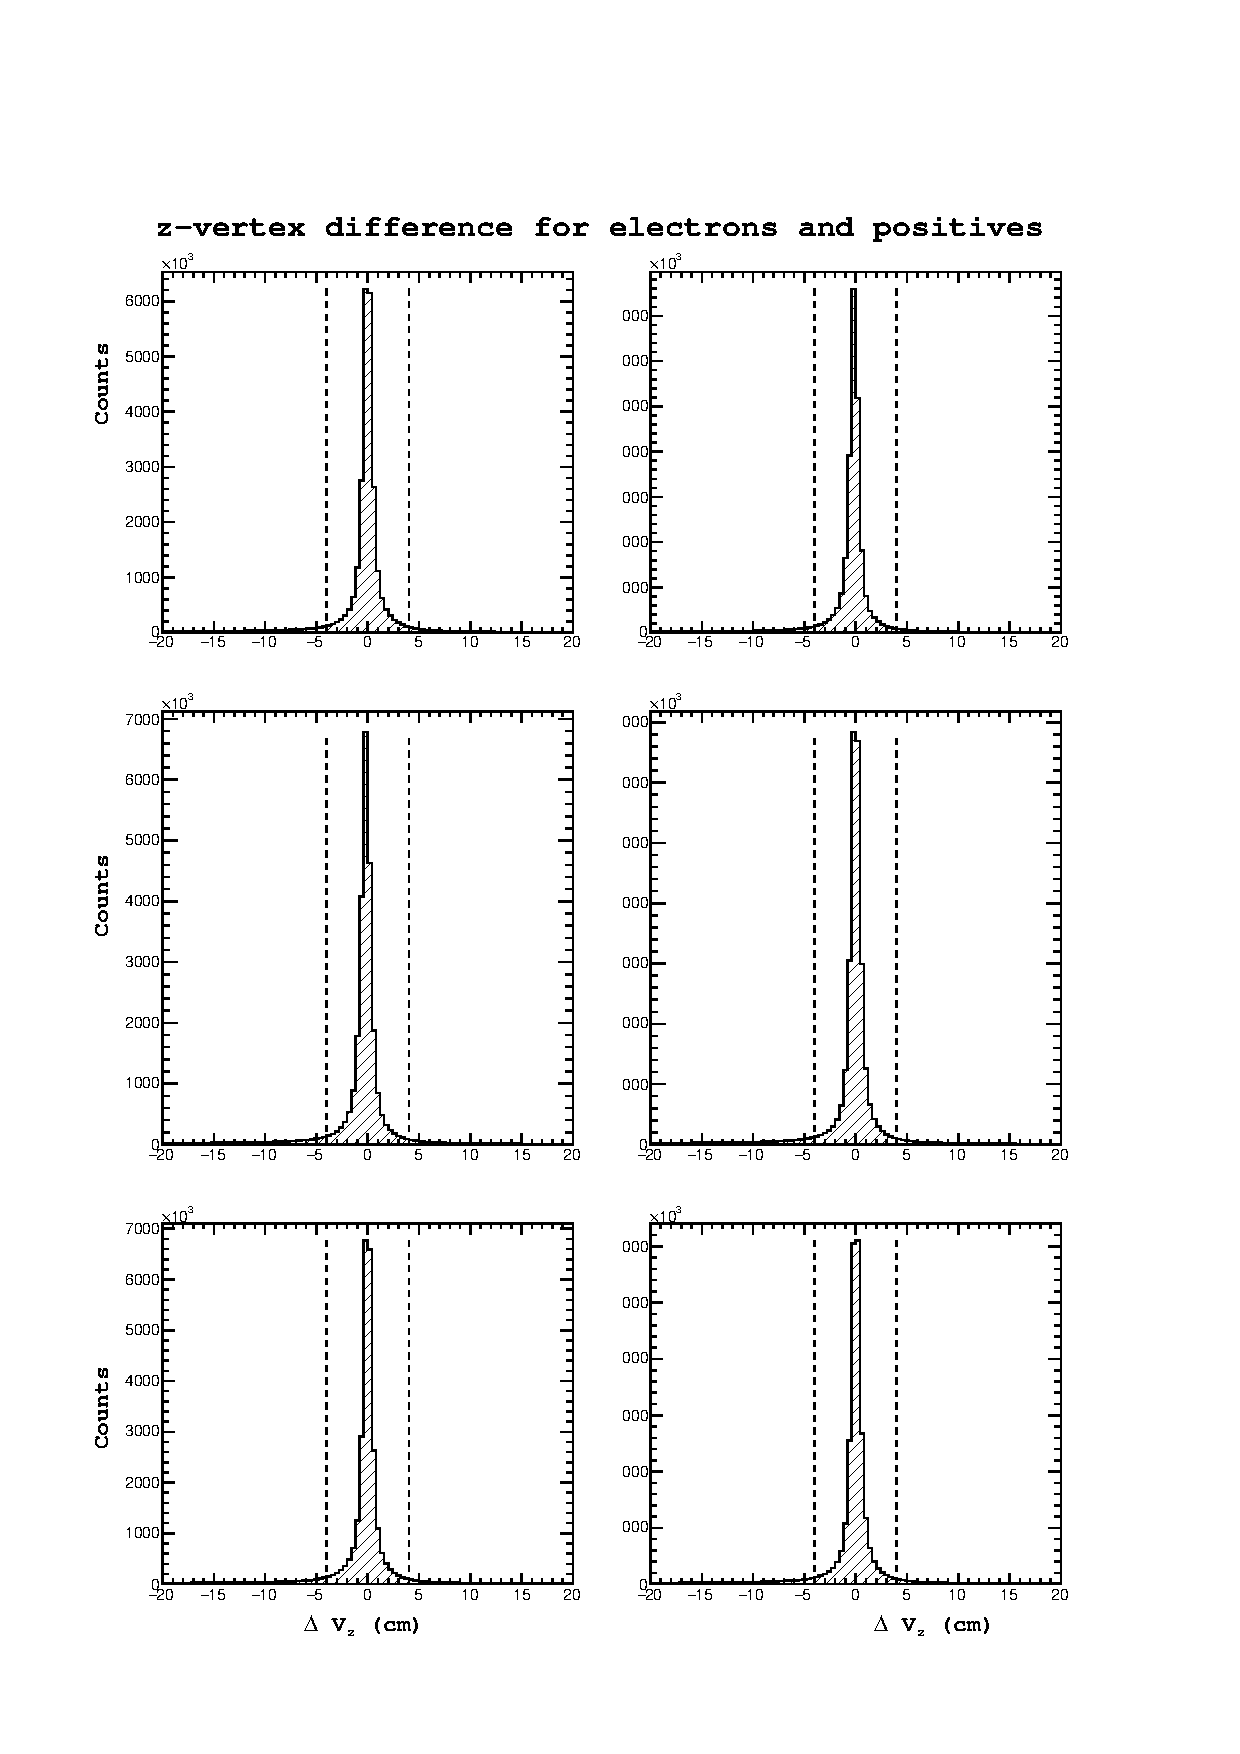
\includegraphics[width=10cm]{image/dvz.pdf}
    \caption{Shown above: The difference between the z-vertex position between detected electrons and positive tracks.}
  \end{center}
\end{figure}

\begin{figure}
  \begin{center}
    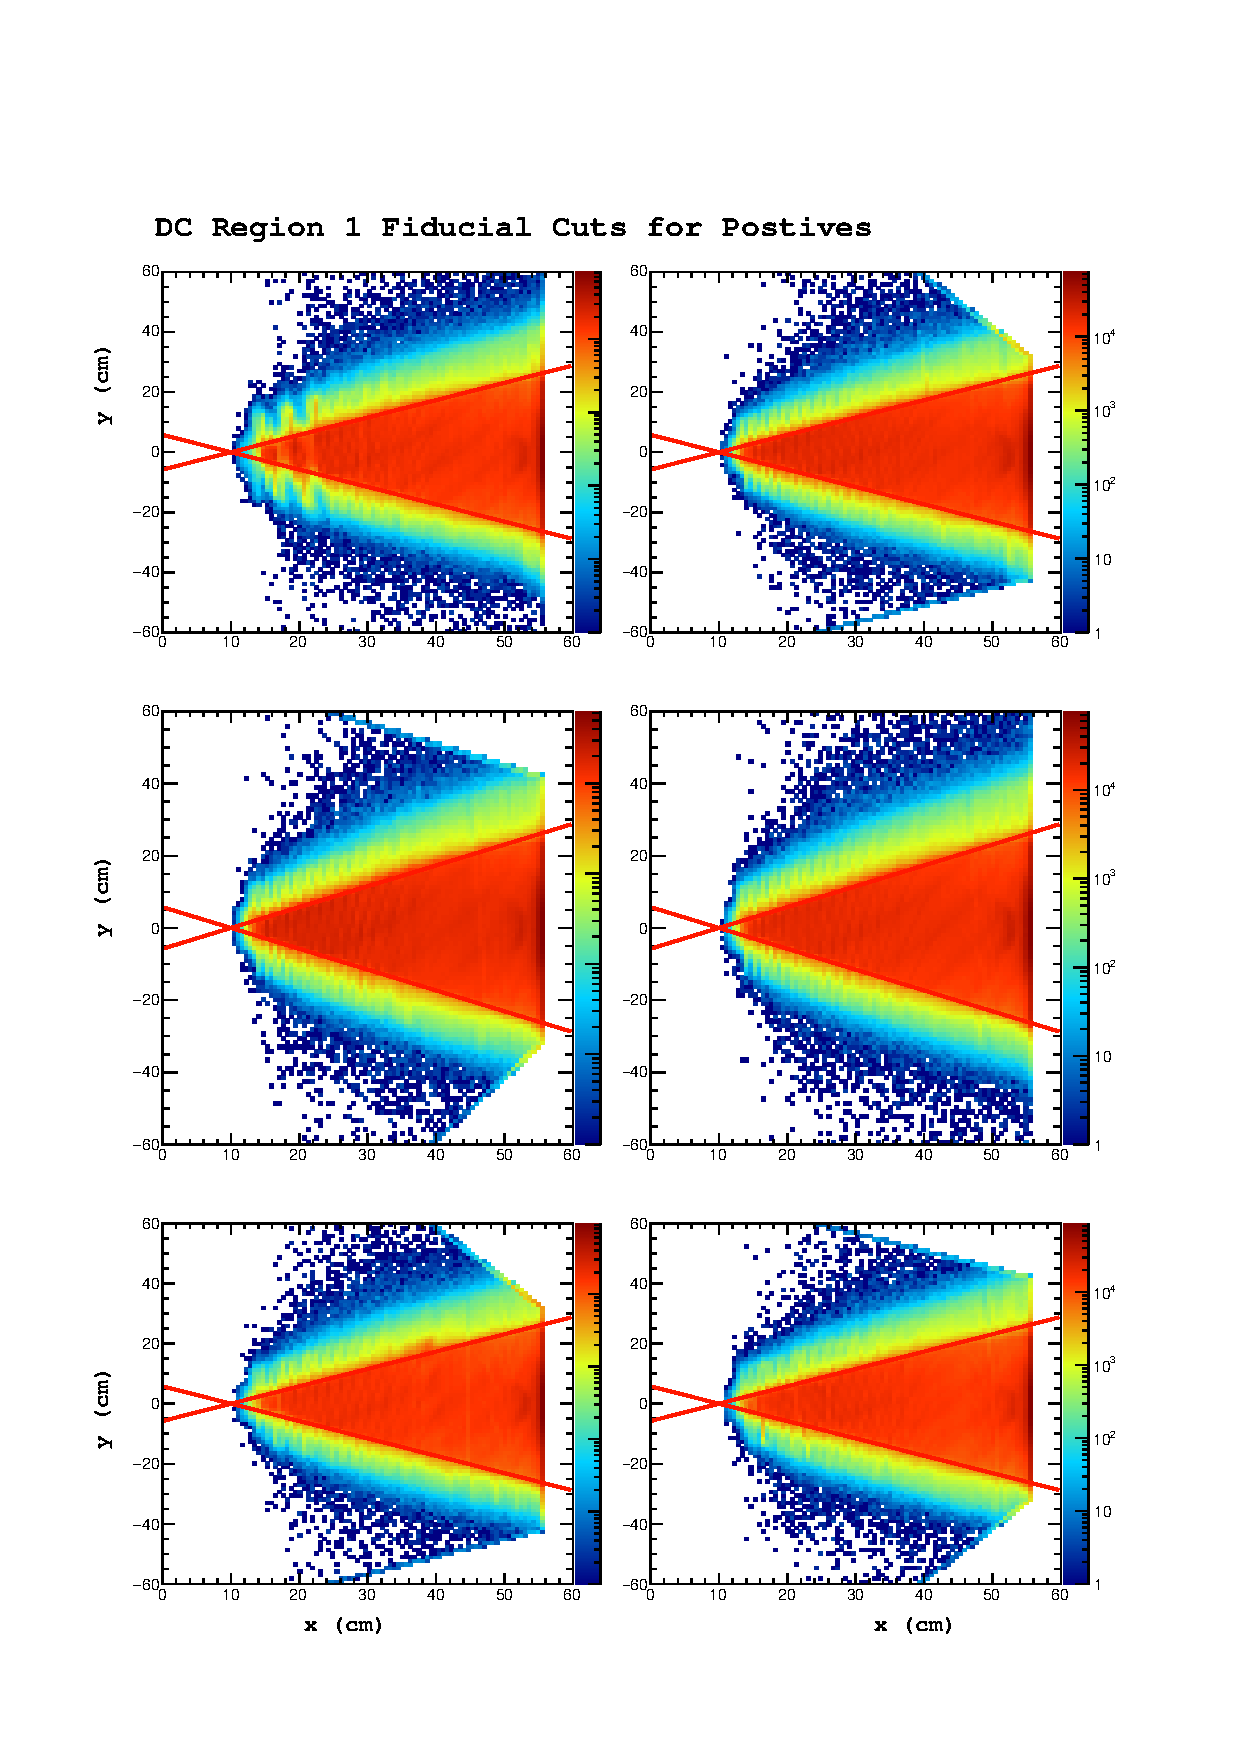
\includegraphics[width=10cm]{image/fid.pdf}
    \caption{Shown above: Positive track hits on the region 1 drift chamber, events falling between the red lines are kept for analysis.}
  \end{center}
\end{figure}


%\begin{figure}
%  \begin{center}
%    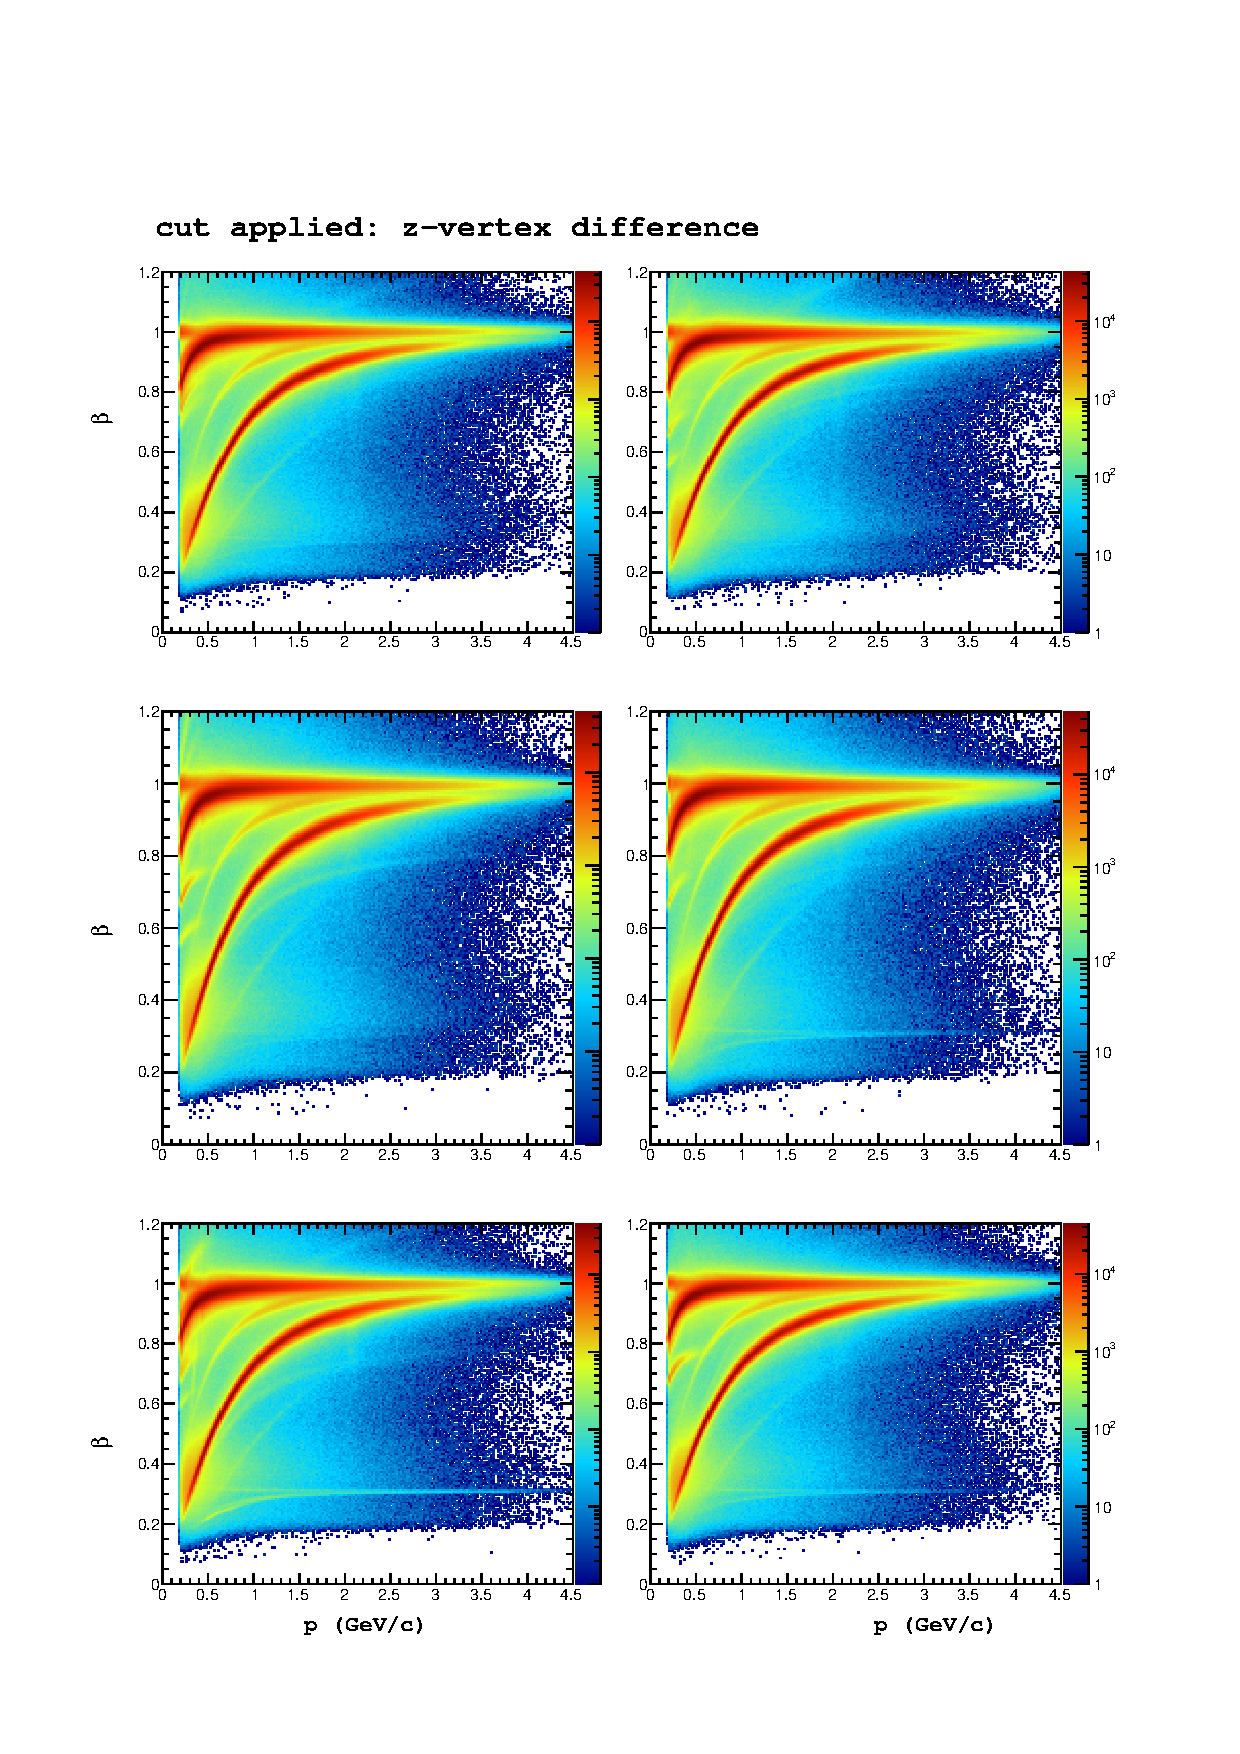
\includegraphics[width=10cm]{image/p_beta_dvz.pdf}
%    \caption{Shown above: }
%  \end{center}
%\end{figure}

%\begin{figure}
%  \begin{center}
%    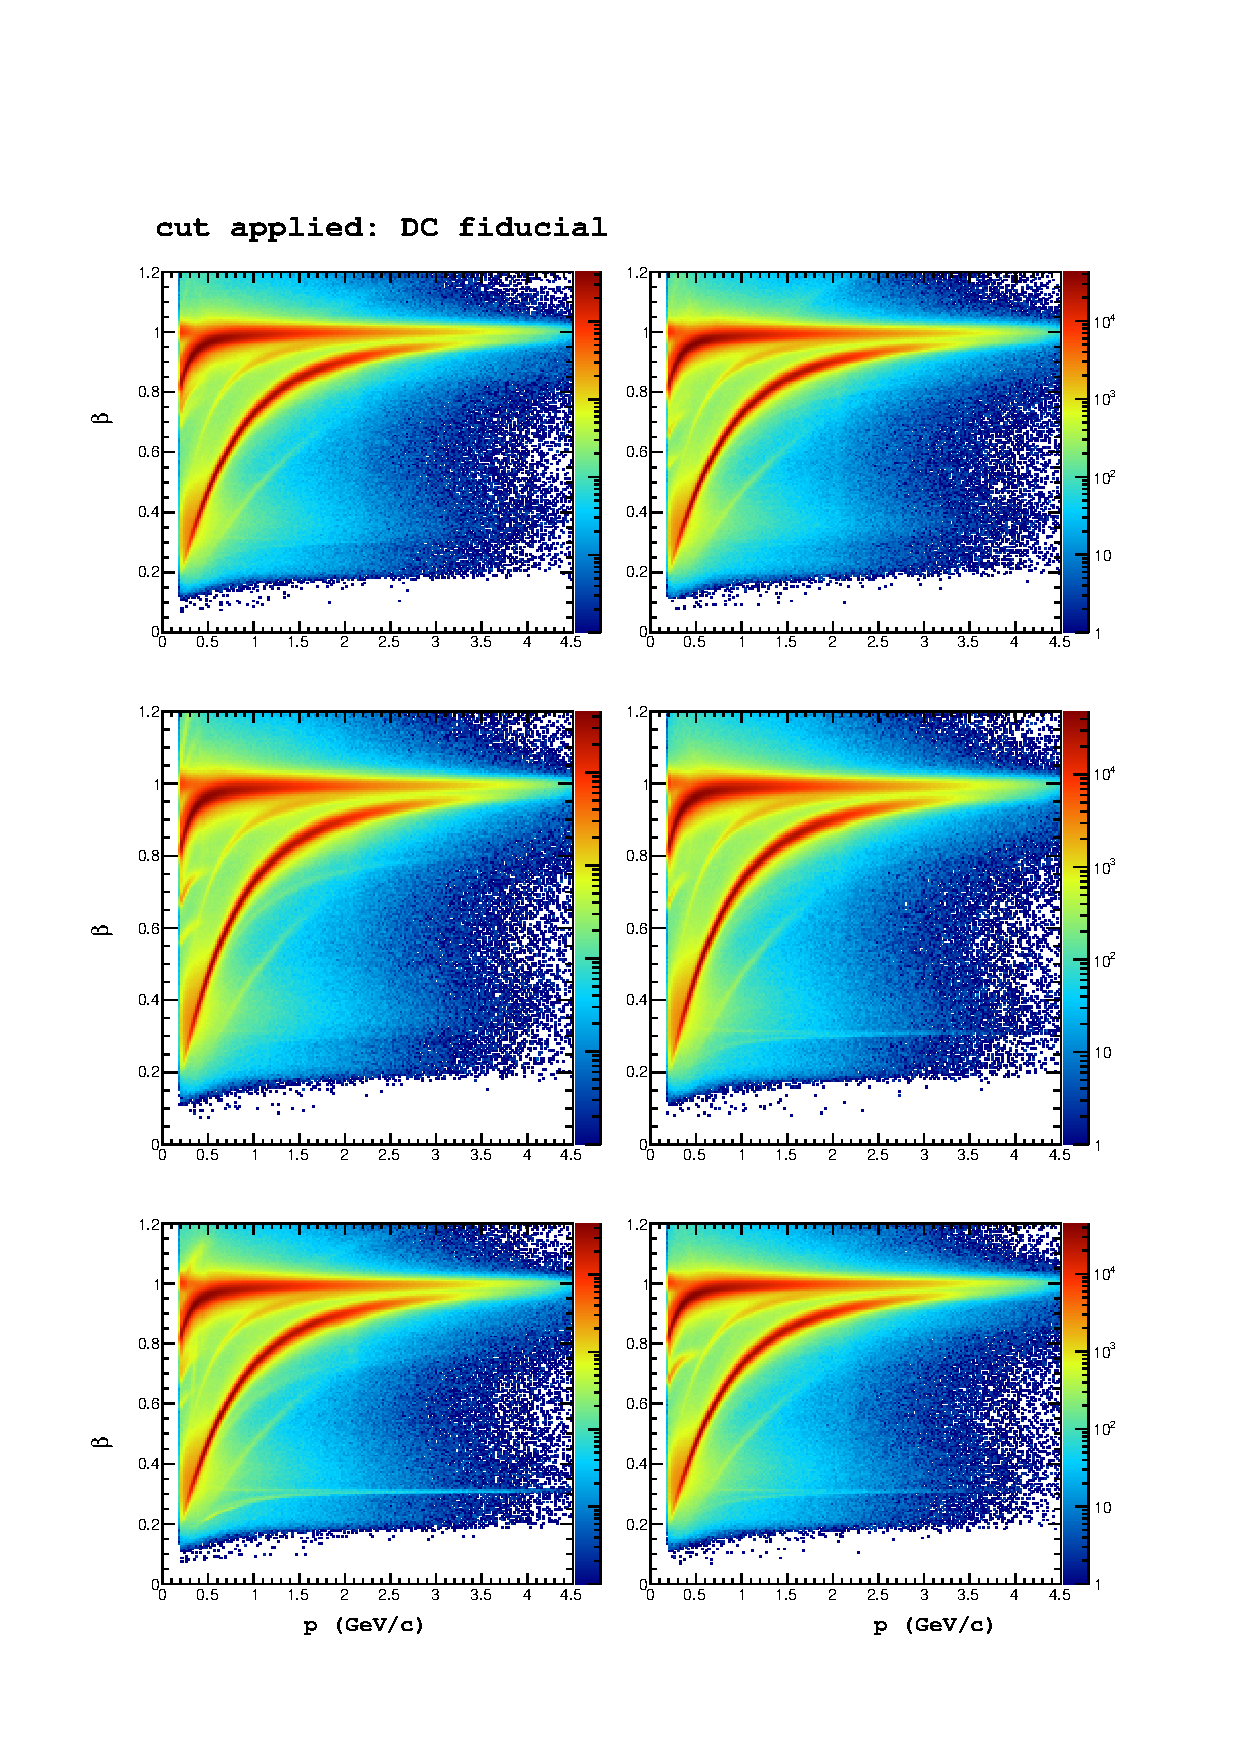
\includegraphics[width=10cm]{image/p_beta_fid.pdf}
%    \caption{Shown above: }
%  \end{center}
%\end{figure}
